\chapter{Digital Signal Processor}
\label{chapter:dsp}

%----------------------------------------------------------------------------------------
%	Section
%----------------------------------------------------------------------------------------

\section{ADSP-BF548 EZ-KIT Lite}

This section primarily summarizes the hardware-related information that helps developers write more robust and efficient C code.

%--------------------------------------------
%--------------------------------------------

\subsection{Hardware Architecture}

\textbf{Audio Codec} in charge of sampling speech and \textbf{Memory Hierarchy} that restricts the storage of variables are highly significant to the implementation on the DSP board.

%--------------------------------------------

\subsubsection{Audio Codec}
An Analog Devices AD1980 audio codec is the audio interface of the EZ-KIT Lite. The codec connects to multiple audio connectors (3.5 mm) which allow us to get audio in and out. These connectors can be easily found at the bottom left corner of the board.

\begin{figure}[H]
\centering
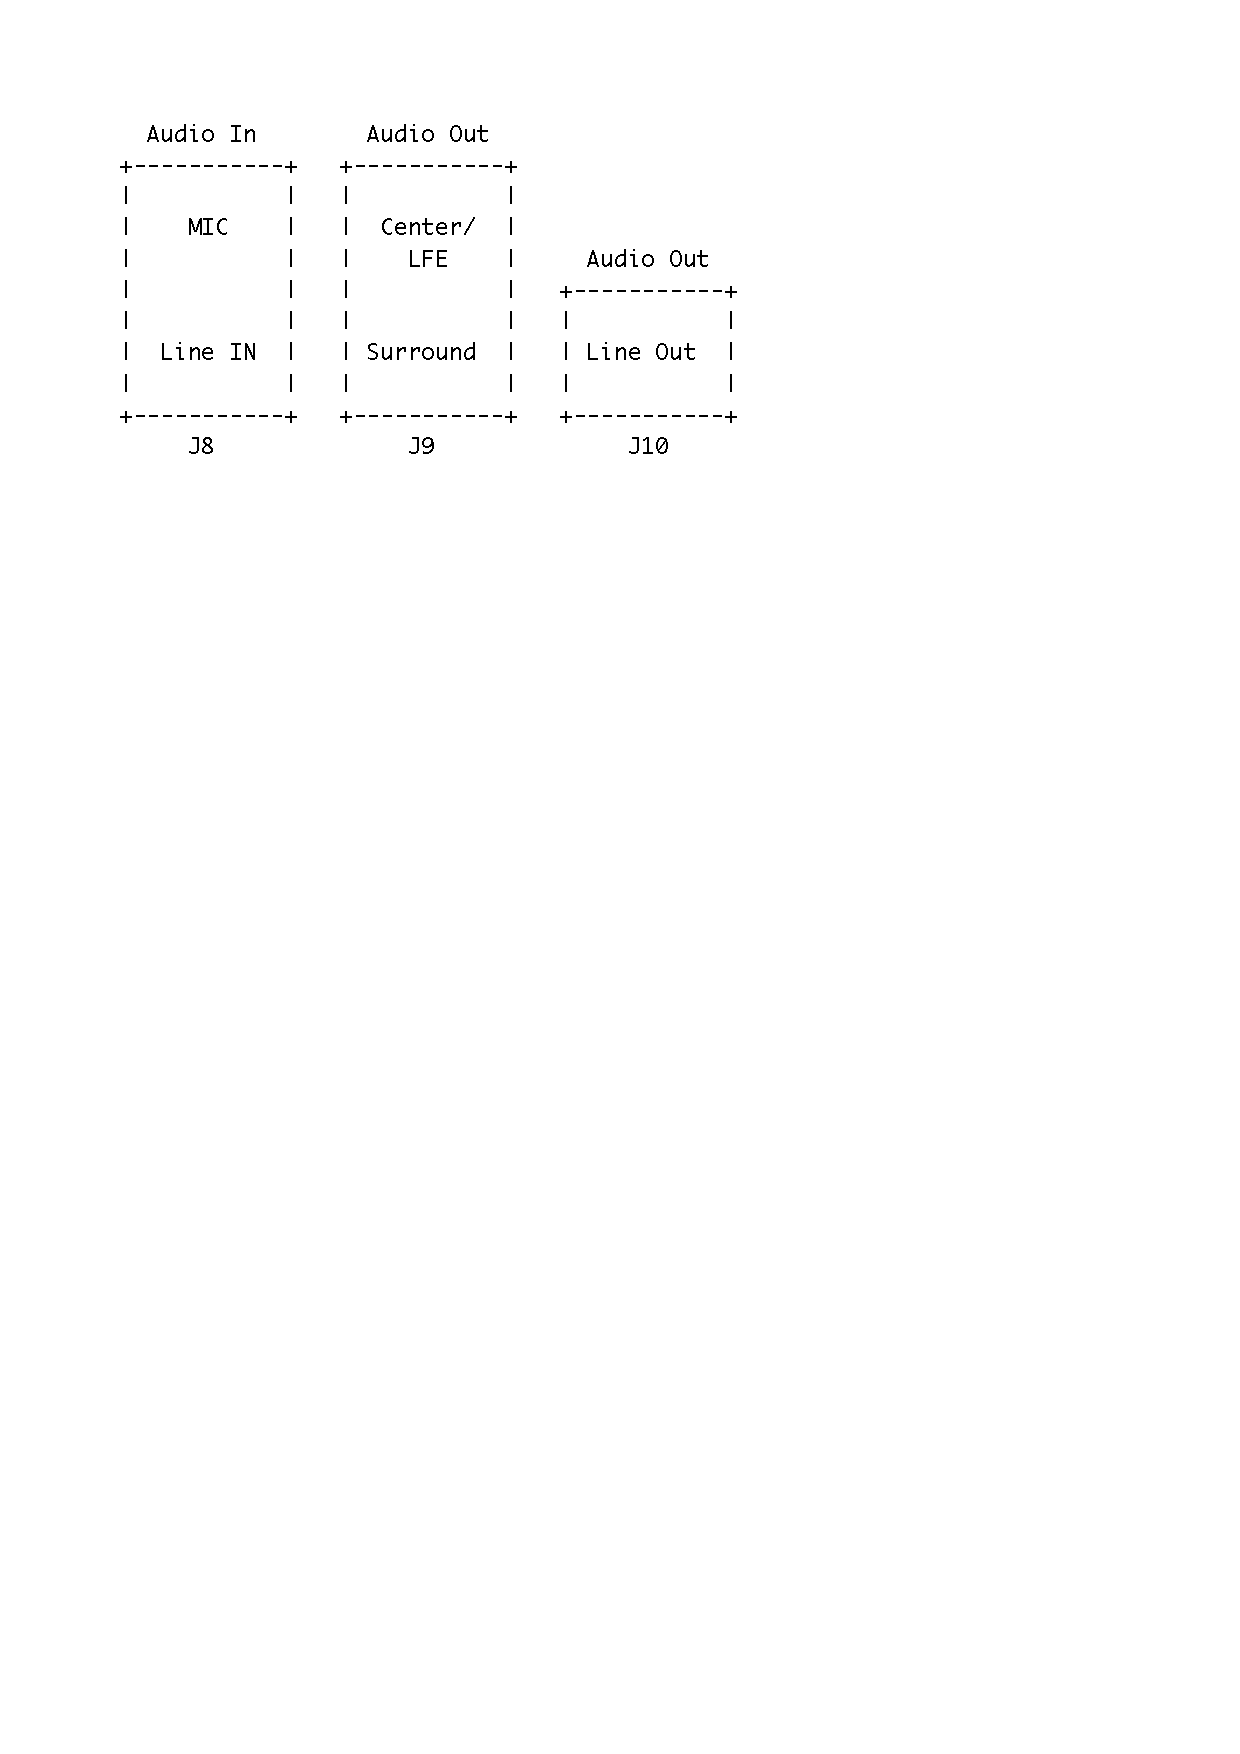
\includegraphics[width=3in]{ang/audio-connectors}
\caption{Audio Connectors}
\label{audio-connectors}
\end{figure}

Fig. \ref{audio-connectors} illustrates that the top location of \texttt{J8} is for a stereo microphone and the bottom location is for a stereo line in. According to Fig. \ref{AD1980-schematic}, the difference between \texttt{MIC} and \texttt{LINE IN} is signals via \texttt{MIC} will be pre-amplified. The preamp gain is collaboratively controlled by \texttt{MIC} Volume Register (\texttt{AD1980\_REG\_MIC\_VOL\_CTRL}) and Miscellaneous Control Bit Register (\texttt{AD1980\_REG\_MIC\_VOL\_CTRL}) \cite{AC97-codec}. In addition, it can be clearly seen that AD1980 can only sample 2 channels at any given moment due to the RECORD SELECTOR multiplexer. Thus, we decide to input noisy command and noise via the left / right channel of \texttt{MIC} respectively.

\begin{figure}[H]
\centering
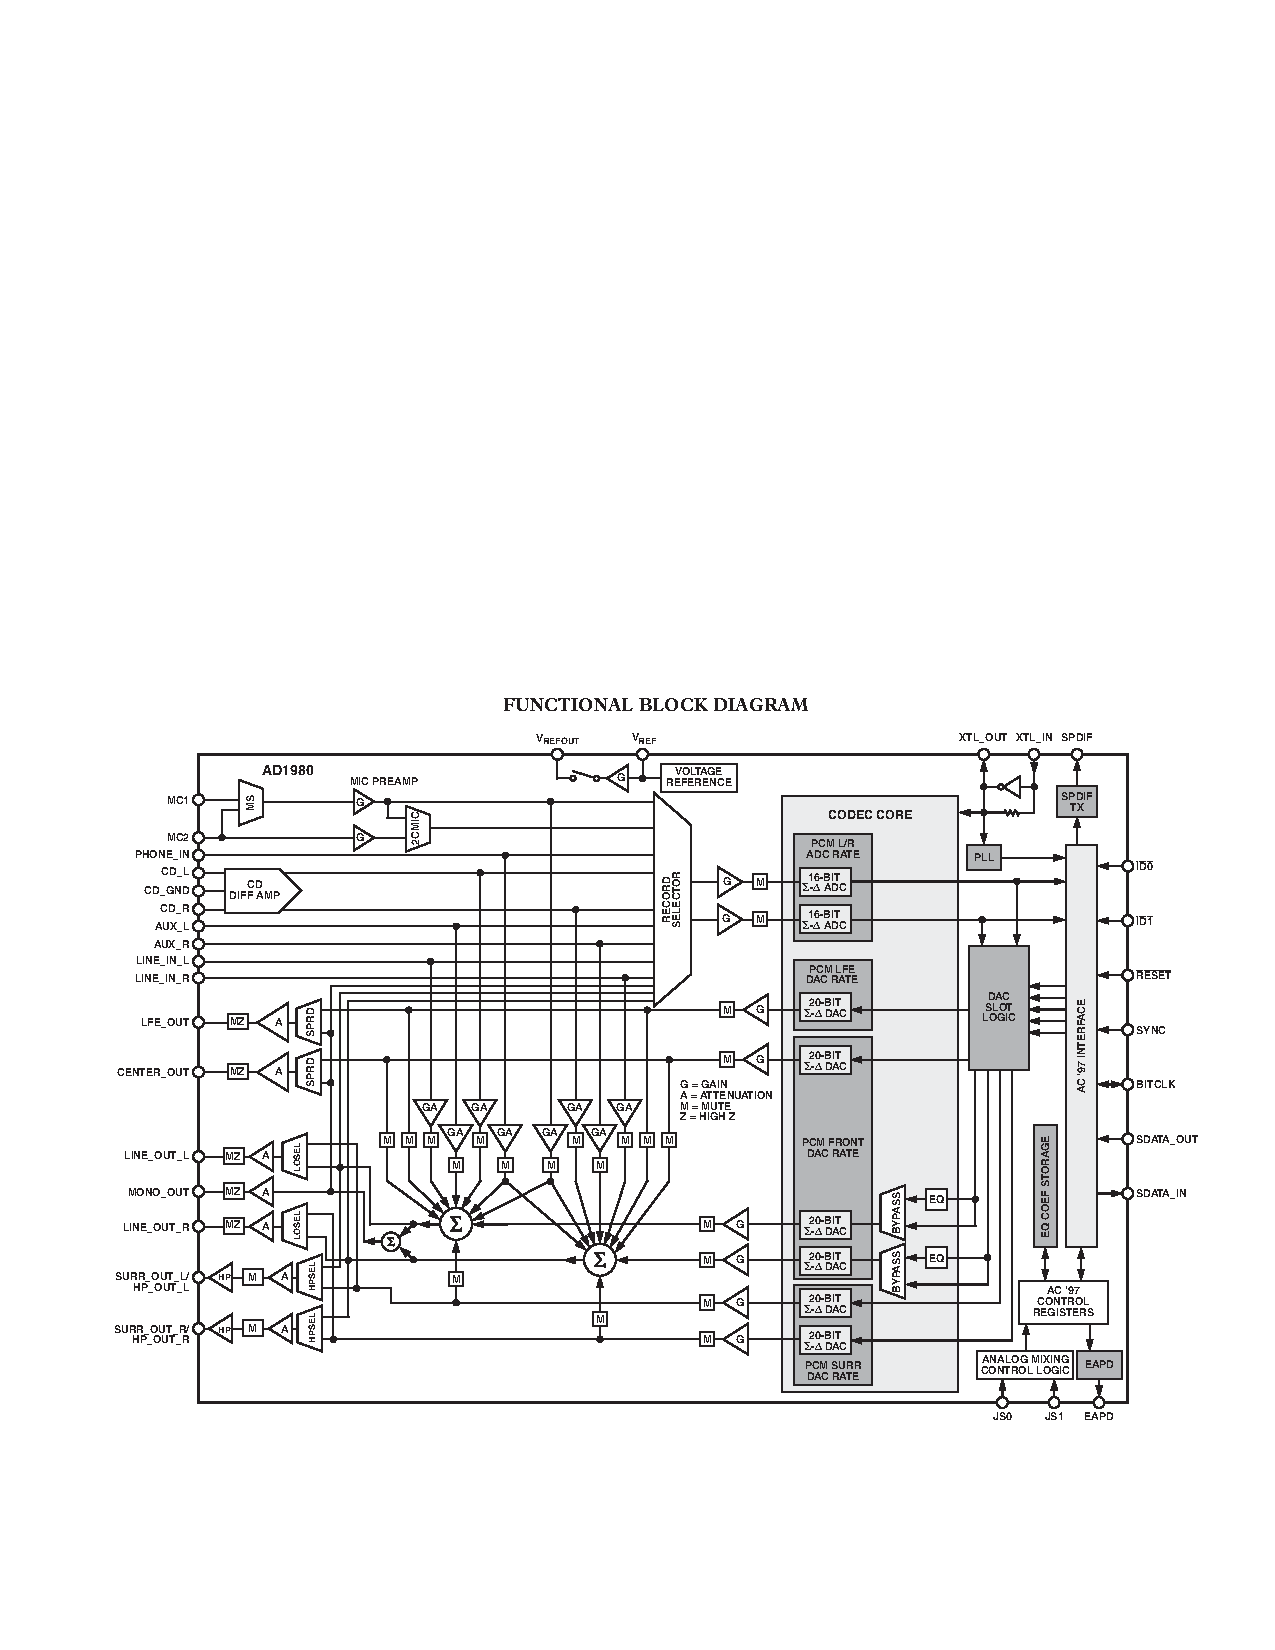
\includegraphics[width=6in]{ang/AD1980-schematic}
\caption{AD1980 Functional Block Diagram}
\label{AD1980-schematic}
\end{figure}

%--------------------------------------------

\subsubsection{Memory Hierarchy}
The ADSP-BF548 processor supports a hierarchy of three synchronous memories.\\

Internal L1 memory offers two 32 KB SRAM banks for data \cite{bf54x-hardware}. ``L1 memory is the highest-performing memory available to the Blackfin core and can be accessed at core clock speeds.''\cite{start-with-bf548}\\

Internal L2 memory consists of a single 128 KB area of SRAM. ``L2 is somewhat lower-performing than L1, requiring two core clock cycles for access.'' L2 provides larger capacity accompanied by higher latency. \cite{start-with-bf548} Totally, 32768 variables of 32-bit data type (e.g. \texttt{float} and \texttt{fract32}) can be stored in L2.\\

External memory is a 64 MB DDR SDRAM that exists external to the processor mounted on the DSP board. ``External memory operates synchronously with the processor's system clock rather than the core clock, causing access time to SDRAM to be relatively slower than to L1 or L2 memory.''\cite{start-with-bf548} 64 MB (67108864 bytes) is enormous given that each \texttt{float} / \texttt{fract32} variable occupies 4 bytes. Hence, we will pre-compute reusable coefficients as long as fetching them from external memory is faster than computing them. In fact, L1 \& L2 are big enough to store these coefficients, decisions will be elaborated in \fullref{section:c_program}.

%--------------------------------------------
%--------------------------------------------

\subsection{Data Types}

\subsubsection{Directly Supported Data Types}

Table \ref{fixed-point-data-types} (in appendix on page \pageref{fixed-point-data-types}) and Table \ref{floating-point-data-types} summarize the ten scalar data types directly supported by the complier.\\

Table \ref{main-fixed-point-data-types} as a subset of Table \ref{fixed-point-data-types} lists main fixed-point data types. Note that \texttt{long} is equivalent to \texttt{int}. We use 8-bit \texttt{unsigned char} when manipulating GPIO (\textit{General Purpose I/O}) registers.

\begin{table}[H]
\centering
\caption{Main Fixed-Point Data Types}
\label{main-fixed-point-data-types}
\begin{tabu} to \textwidth {XXXX}
\toprule
Type &Size &Min &Max\\
\hline
\texttt{unsigned char} &8-bit &0 &255\\
\hline
\texttt{short} &16-bit &-32,768 &32,767\\
\hline
\texttt{int} &32-bit &-2,147,483,648 &2,147,483,647\\
\hline
\texttt{long} &32-bit &-2,147,483,648 &2,147,483,647\\
\bottomrule
\end{tabu}
\end{table}

Table \ref{floating-point-data-types} summarizes properties of floating-point data types. Note that \texttt{double} is equivalent to \texttt{float}. Value ranges are computed based on the internal representation of single-precision floating-point numbers. Details are provided in appendix on page \pageref{subsection:float-data-type}. We have also shown \texttt{float} has a precision of $\log_{10}(2^{24}) \approx 7.225$ decimal digits in the appendix. This deduction is significant to exporting model and coefficients from MATLAB.

\begin{table}[H]
\centering
\caption{Floating-Point Data Types}
\label{floating-point-data-types}
\begin{tabu} to \textwidth {XXX}
\toprule
Type &Size &Range\\
\hline
\texttt{float} &32-bit &$\pm 1.18 \times 10^{-38}$ to $\pm 3.4 \times 10^{38}$\\
\hline
\texttt{double} &32-bit &$\pm 1.18 \times 10^{-38}$ to $\pm 3.4 \times 10^{38}$\\
\bottomrule
\end{tabu}
\end{table}

The smallest denormalized number has a marked impact on small probability calculation. For instance, the emission probability can easily become smaller than $e^{-200} = 1.3839 \times 10^{-87}$. Fortunately, all computation involved between probabilities are multiplications, hence we take natural logarithm before conducting multiplications and convert all multiplications into additions based on the property of logarithm (\ref{log-property}).

\begin{equation}
\label{log-property}
\ln(xy) = \ln(x) + \ln(y)
\end{equation}

%--------------------------------------------

\subsubsection{Fractional Data Types}

Fractional data types \texttt{fract16} and \texttt{fract32} can be represented as \texttt{short} and \texttt{int} respectively. Fig. \ref{bf_fract_represent} shows the internal representation of \texttt{fract16} and \texttt{fract32} (from National Instruments). Table \ref{fractional-data-types} lists the main properties of fractional data types. \texttt{fract32} has higher precision (assuming no overflow or underflow) and higher processing speed (due to fixed-point arithmetic) than \texttt{float}. Hence, \texttt{fract32} variables are widely utilized when implementing the algorithms introduced in \fullref{chapter:speech-processing}.

\begin{figure}[H]
\centering
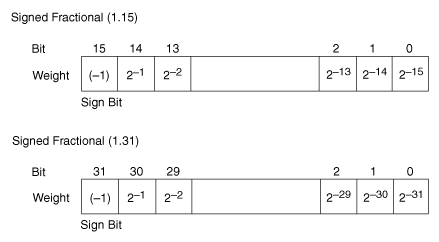
\includegraphics[width=3in]{ang/bf_fract_represent}
\caption{Internal Representation of Fractional Data Types}
\label{bf_fract_represent}
\end{figure}

\begin{table}[H]
\centering
\caption{Fractional Data Types}
\label{fractional-data-types}
\begin{tabu} to \textwidth {XXXX}
\toprule
Type &Size &Range &Resolution\\
\hline
\texttt{fract16} &16-bit &$-1$ to $1 - 2^{-15}$ &$2^{-15}$\\
\hline
\texttt{fract32} &32-bit &$-1$ to $1 - 2^{-31}$ &$2^{-31}$\\
\bottomrule
\end{tabu}
\end{table}

%--------------------------------------------
%--------------------------------------------

\subsection{CrossCore Embedded Studio}

During ELEN90058 \textit{Signal Processing} and ELEN90052 \textit{Advanced Signal Processing} workshop sessions, we used CrossCore\textsuperscript{\textregistered} Embedded Studio to compile and debug code for Blackfin DSP board. Basing on Eclipse, CCES exploits the ecosystem of third-party tools already available to Eclipse developers. Thus, plenty of convenient functions such as plotting arrays of data are available to users \cite{erik-cces}\cite{cces-faq}. CCES could be an ideal substitution for VisualDSP++.\\

However, the AD1980 Audio Codec on ADSP-BF548 EZ-Kit Lite Board is not supported with CCES \cite{cces-ad1980}. Analog Devices engineer Craig Gilchrist explained in \textit{EngineerZone} support community that they do not have a driver for the AD1980 Codec with CCES. In addition, he recommended AD1836 Audio Codec instead \cite{BF548-BSP}.\\

Considering the project budget and potential risk, we eventually decided to stick on VisualDSP++ 5.1.2.

%----------------------------------------------------------------------------------------
%	Section
%----------------------------------------------------------------------------------------

\section{Software Development}

\subsection{Software Process}
We develop the software system of our project according to the following set of activities.
\begin{enumerate}
\item Determine system specification.
\item Design algorithm in MATLAB.
\item Optimize program efficiency in MATLAB, e.g. pre-computing reusable coefficients, taking advantage of symmetry, scaling data in order to use fixed-point arithmetic.
\item Develop evolutionarily. Implementation and validation are interleaved.
\begin{enumerate}
	\item Implement each function in C language on DSP board.
	\item Validate each function by comparing the outcomes calculated by DSP with the expected results from MATLAB. Round off errors are allowed but differences are supposed to be within precision tolerance.
\end{enumerate}
\item Adjust algorithm in MATLAB if the original design is infeasible to implement due to precision and speed restriction of DSP board.
\item Implement algorithms for real-time processing.
\item Tune performance by optimizing efficiency and improving accuracy.
\end{enumerate}

%--------------------------------------------
%--------------------------------------------

\subsection{Revision Control \& Source Code Management}

We host and manage our code on GitHub which helps us control revisions and manage source code better. Reviewing what has been modified before committing the change to the server minimizes the possibility of misoperation. Besides, we hope our work could contribute to the open-source community inversely because we have benefited from open-source spirit so much.\\

Project Repository: \url{https://github.com/leeang/Word-Recognition}

%----------------------------------------------------------------------------------------
%	Section
%----------------------------------------------------------------------------------------

\section{C Program}
\label{section:c_program}

In addition to the experience gained in workshops, \cite{TuningCSourceCode} provides official guidance for optimizing C program execution efficiency. During implementation, we reduce floating-point arithmetic as much as possible and try to avoid integer division in loops.

\subsection{Audio\_Loopback}

Analog Devices provides an example named \texttt{Audio\_Loopback} which simply copies the sampled and quantized audio input to the audio output in real-time. This example is available in the /\texttt{Drivers}/\texttt{AudioCodec} folder under VisualDSP++ installation directory. This framework initializes the codec AD1980 via the device manager and will invoke an interrupt callback function when the inbound buffer is full.\\

This example project helps us spend more time on our main quest instead of configuring hardware environment from scratch. Original \texttt{.h} and \texttt{.c} files are added to the project. Some codes are added to \texttt{main} and \texttt{AD1980Callback} function to initialize the recognition system and associate the functions properly.
\begin{enumerate}
\item \texttt{header.h} defines all constants and global variables.
\item \texttt{function.c} includes all original functions.
\item \texttt{model.h} contains speech models exported from MATLAB.
\item \texttt{mel\_filter.h} incorporates precomputed Mel-filter bank gain.
\end{enumerate}

%--------------------------------------------
%--------------------------------------------

\subsection{Buffering}

We set the length of segment buffer as 6000 data points, i.e. interrupt callback function is called every $6000 / 16000 = 0.375$ seconds. Time-consuming LMS based filter works every interrupt and noise-reduced command is cached in a buffer of 48000 data points. Speech signal processing and recondition routine run once when the eighth interrupt comes.

%--------------------------------------------
%--------------------------------------------

\subsection{Pre-emphasis}

It is easy to prove that filter characteristic represented by (\ref{shelving-filter}) will not change if coefficients $a_i$ and $b_i$ are uniformly scaled. Some pre-emphasis filter coefficients (\ref{shleving-coef}) are beyond the fractional data types domain $[-1, 1]$. Hence, the coefficients are scaled by $\lambda$ before converting them from \texttt{float} to \texttt{fract32}.\\

We choose $\lambda = \frac{1}{4}$ primarily because $\frac{1}{a_0} = \frac{1}{\lambda} = 4$ which is a power of 2. In terms of fixed-point data types, left shifting 2 bits is equivalent to multiplying by $\frac{1}{a_0} = 4$ but left shifting is more efficient. Besides, $\lambda = \frac{1}{2}$ is not small enough while $\lambda = \frac{1}{8}$ leads to loss in precision. $a_i \in [-1, 1]$ and $b_i \in [-1, 1]$ for $\forall i = 0, 1, 2$ when $\lambda = \frac{1}{4}$.

\begin{align*}
&\begin{cases}
a_0 = \frac{1}{4} = 0.25\\
a_1 = \frac{-1.523796}{4} = -0.380949\\
a_2 = \frac{0.649345}{4} = 0.162336
\end{cases}
&\begin{cases}
b_0 = \frac{1.861856}{4} = 0.465464\\
b_1 = \frac{-3.102851}{4} = -0.775712\\
b_2 = \frac{1.366544}{4} = 0.341636
\end{cases}
\end{align*}

Filter coefficients are converted into \texttt{fract32} once by \texttt{calc\_shelving\_coef()} function when initializing the system. Finally, all computations in \texttt{pre\_emphasis()} function are fixed-point arithmetic.

%--------------------------------------------
%--------------------------------------------

\subsection{Hamming Window}

For the window length $N = 512$, Hamming window weight $w[n]$ has 512 elements. Table \ref{clocks-hamming} summarizes the efficiency of different methods to obtain $w[n]$. $512/2 = 256$ (due to symmetry) \texttt{fract32} data points occupy 1 KB. There is no reason to recompute them every time. Considering they are most frequently used (180 times per 3-second recording), we store them in the fastest L1 memory. During the initialization session, \texttt{calc\_hamming\_coef} function pre-computes them and converts them into \texttt{fract32}. All computations in \texttt{hamming()} function are fixed-point arithmetic.

\begin{table}[H]
\centering
\caption{Efficiency of Approaches to Obtain $w[n]$}
\label{clocks-hamming}
\begin{tabu} to \textwidth {XXX}
\toprule
Action &clocks &time elapsed\\
\hline
compute &607471 &1.012452 ms\\
\hline
fetch from L1 &8731 &0.014552 ms\\
\hline
fetch from L2 &12827 &0.021378 ms\\
\hline
fetch from external memory &30878 &0.051463 ms\\
\bottomrule
\end{tabu}
\end{table}

%--------------------------------------------
%--------------------------------------------

\subsection{Thresholds}
\label{subsection:dsp-thresholds}
\subsubsection{Frame Energy}

The energy of frame $j$ is defined in (\ref{eq:frame-energy}) on page \pageref{eq:frame-energy}. We have known the amplitude of a data point $-1 \le s_j[n] \le 1$, thus the power of this point $(s_j[n])^2 \le 1$. The energy of a frame is the sum of $N$ power points. We invoke intrinsic function \texttt{add\_fr1x32()} when performing addition of 32-bit fractional data. Although the energy is possibly larger than 1, because intrinsic functions support saturation arithmetic that prevents overflow \cite{gan2007embedded}. That is, the addition function will return 1 if the original outcome exceeds 1. Given the threshold set by us is smaller than 1, as long as the variable becomes saturated, the frame energy will be definitely higher than the threshold. Hence, saturation will not influence the threshold decision.

%--------------------------------------------
%--------------------------------------------

\subsection{MFCC extraction}
\subsubsection{Power Spectrum}

We have known that the DFT of a $N$-point real sequence can be obtained from one $\frac{N}{2}$-point complex-valued DFT and additional computations (from ELEN90058 \textit{Signal Processing} lecture slides by Erik \textsc{Weyer}). VisualDSP++ has a built-in function called \texttt{rfft\_fr32()} to exploit this property.\\

\texttt{rfft\_fr32()} function takes 7 arguments. The first two are time domain real sequence input and spectrum output. The third one is the twiddle table calculated once by \texttt{twidfftrad2\_fr32()} function during system initialization. The fourth parameter is the twiddle stride that should be set to 1 because the twiddle table is tailored to this FFT. The fifth argument is the FFT size which equals the window length $N = 512$. The last two are block exponent and scaling method. We select dynamic scaling mode that will inspect intermediate results and only apply scaling where required to prevent overflow. In this mode, precision can be better preserved than in static scaling method, although inspections leads to an negative impact on performance. The block exponent returned will be the number of times that the function scales the intermediate set of results.\\

Once the spectrum is obtained, we invoke \texttt{cabs\_fr32()} function to compute the magnitude of each data point (data type: \texttt{complex\_fract32}), the product of the magnitude and itself is the power of each point.

%--------------------------------------------

\subsubsection{Bank Filtering \& Log Scaling}

Fig. \ref{bank_filter_demostration} depicts the process to compute $X_j[m]$ of bank $m = 9$ based on (\ref{eq:mel-filter}) on page \pageref{eq:mel-filter}. In subplot 1, each power data point $\hat{S}_j[k]$ (\textcolor{gold_matlab}{gold circle $\circ$}) is multiplied by the corresponding gain $H_{mel}[m, k]|_{m=9}$ (\textcolor{orange_matlab}{orange asterisk $*$}). Filtered power data points are shown in subplot 2 by \textcolor{orange_matlab}{orange cross $\times$}. Thereby, the sum of all filtered power data points is the energy $X_j[m]$ within filter bank $m = 9$.

\begin{figure}[H]
\begin{minipage}[t]{0.5\linewidth}
\centering
\minipageplot{ang/bank_filter_demostration}
\caption{Bank Filtering Demonstration}
\label{bank_filter_demostration}
\end{minipage}
\begin{minipage}[t]{0.5\linewidth}
\centering
\minipageplot{ang/mel_filter_bank_gain}
\caption{Gain of Each Point in Each Bank}
\label{mel_filter_bank_gain}
\end{minipage}
\end{figure}

Fig. \ref{bank_filter_demostration} also shows that bank $m=9$ only intersects with 16 data points in power spectrum because gain for other points are all zero. We plot the gain of each data point for each bank in Fig. \ref{mel_filter_bank_gain}, grayscale represents the value of gain. We find the same situation for all banks. Directly computing $H_{mel}[m, k]$ results in a $k \times m$ sparse matrix (white blocks stand for zeros).\\

In order to diminish the processing time by pre-computing and eliminating the useless operations with zeros, we design a special storage structure for this sparse matrix. One array for storing non-zero values in linear shape and one array for storing corresponding offset for each bank. One array for storing at which $k$ gain becomes non-zero (\textcolor{red}{red dashed-line arrows}) and one-array for storing the length of each grayscale block (\textcolor{orange_html}{orange solid-line arrows}).\\

Gains are converted into \texttt{fract32} by \texttt{calc\_bank\_gain()} function during system initialization. Power cepstrum data points are converted back to \texttt{float} in case of saturation before summation that evaluates the total power within each bank. We no longer insist on fixed-point arithmetic because
\begin{enumerate}
\item only 30 - 50 frames (out of 180 frames) are passed to MFCC;
\item precision error will be accumulated;
\item log scaling in the next step will be done with the aid of \texttt{float} type \texttt{log()} function;
\item outcome of logarithm ranges widely.
\end{enumerate}

%--------------------------------------------

\subsubsection{Discrete Cosine Transform}

We define
\begin{equation}
\label{eq:dct-coef}
H_{dct}[n, m] = \sqrt{\frac{2}{M}} \cos \left( \frac{\pi}{M} (m - 0.5) (n-1) \right)
\end{equation}
where $n = 1, 2, \dots, F$ and $m = 1, 2, \dots, M$.\\

Thereby, (\ref{eq:dct}) becomes
\begin{equation}
\label{eq:dct-coef-form}
\hat{C}_j[n] = \sum^{M}_{m=1} \hat{X}_j[m] H_{dct}[n, m] \quad n = 1, 2, \dots, F
\end{equation}

It can be proven that for even $M$ and odd $F$
\begin{equation}
H_{dct}[n, m] =
\begin{cases}
H_{dct}[n, M-m+1] & n = 1, 3, \dots, F\\
-H_{dct}[n, M-m+1] & n = 2, 4, \dots, F-1
\end{cases}
\end{equation}

By utilizing this symmetry, (\ref{eq:dct-coef-form}) can be simplified as
\begin{equation}
\label{eq:dct-symmetric-form}
\hat{C}_j[n] = 
\begin{cases}
\displaystyle\sum^{M/2}_{m=1} (\hat{X}_j[m] + \hat{X}_j[M-m+1]) H_{dct}[n, m] & n = 1, 3, \dots, F\\
\displaystyle\sum^{M/2}_{m=1} (\hat{X}_j[m] - \hat{X}_j[M-m+1]) H_{dct}[n, m] & n = 2, 4, \dots, F-1
\end{cases}
\end{equation}

To calculate $\hat{C}_j[n]$ for each $n$, (\ref{eq:dct-coef-form}) requires $M$ multiplications and $(M - 1)$ additions while (\ref{eq:dct-symmetric-form}) requires $M/2$ multiplications (reduced by 50\%) and $(M - 1)$ additions. Furthermore, only a half precomputed coefficients need to be stored in memory.\\

We pre-compute $H_{dct}[n, m]$ by \texttt{calc\_dct\_coef()} while initializing the system. Table \ref{clocks-dct} summarizes the efficiency of different methods to obtain $H_{dct}[n, m]$. It can be clearly seen that fetching from external memory is even 40 times faster than directly computing.

\begin{table}[H]
\centering
\caption{Efficiency of Approaches to Obtain $H_{dct}[n, m]$}
\label{clocks-dct}
\begin{tabu} to \textwidth {XXX}
\toprule
Action &clocks &time elapsed\\
\hline
compute &172281 &0.287135 ms\\
\hline
fetch from L1 &3889 &0.006482 ms\\
\hline
fetch from L2 &4929 &0.008215 ms\\
\hline
fetch from external memory &9367 &0.015612 ms\\
\bottomrule
\end{tabu}
\end{table}

%----------------------------------------------------------------------------------------
%	Section
%----------------------------------------------------------------------------------------

\section{Improvements on previous work}

\begin{enumerate}
\item first-order FIR pre-emphasis filter is replaced by shelving filter.
\item coefficients that intensively require floating-point computations are precomputed.\\(pre-emphasis, Hamming window and discrete cosine transform)
\item frame energy is calculated in fixed-point arithmetic.
\item Mel bank filter gains are precomputed and stored in an ingeniously designed structure. Meaningless multiplications with zeros are illuminated.
\end{enumerate}
